\begin{table}[h!]
	\centering	
	\begin{tabular}{c|c|c}
		$\phi_r$ & $\phi_l$ & $\phi$ \\
		\hline
		376.0 & 266.0 & 55.0 \\
376.0 & 265.5 & 55.2 \\
376.0 & 265.7 & 55.2 \\

	\end{tabular}
	\caption{Messwerte zur Bestimmung des Innenwinkels $\phi$ in \si{\degree}}
	\label{tab:WinkelPhi}
\end{table}
Mittelwert $\overline{\phi} = \SI{54.8+-0.3}{}
$
\todo[color=red, inline]{Schreibt man Winkel $\varphi$ in \si{\degree} oder $\varphi$ in Grad? Ich finde ersteres hässlich und zweiteres inkonsistent.}

\begin{table}[h!]
	\centering	
	\begin{tabular}{c|c|c|c}
		Wellenlänge $\lambda$ in \si{\nano\meter} & $\Omega_l$ & $\Omega_r$ & $\eta$ \\
		\hline
		406.22 & 11.4 & 252.1 & 60.7 \\
438.65 & 12.1 & 252.0 & 59.9 \\
467.82 & 13.1 & 252.9 & 59.8 \\
479.99 & 8.7  & 254.6 & 65.9 \\
508.58 & 14.1 & 254.6 & 60.5 \\
546.07 & 14.6 & 255.1 & 60.5 \\
578.02 & 15.0 & 255.5 & 60.5 \\
643.86 & 11.2 & 255.9 & 64.7 \\

	\end{tabular}
	\caption{Messwerte zur Bestimmung des Brechwinkels $\eta$ in \si{\degree}}
	\label{tab:WinkelFarben}
\end{table}

\begin{table}[h!]
	\centering	
	\begin{tabular}{c|c|c}
		$\lambda$ in \si{\nano\meter} & $n$ & Fehler $\sigma_n$ \\
		\hline
		406.22 & 1.965 & 0.000 \\
438.65 & 1.959 & 0.000 \\
467.82 & 1.957 & 0.000 \\
479.99 & 1.950 & 0.000 \\
508.58 & 1.947 & 0.000 \\
546.07 & 1.941 & 0.000 \\
578.02 & 1.935 & 0.000 \\
643.86 & 1.919 & 0.000 \\

	\end{tabular}
	\caption{Errechnete Brechzahlen $n$ für jede Wellenlänge $\lambda$}
	\label{tab:Brechzahl}
\end{table}

\begin{figure}
	\centering
	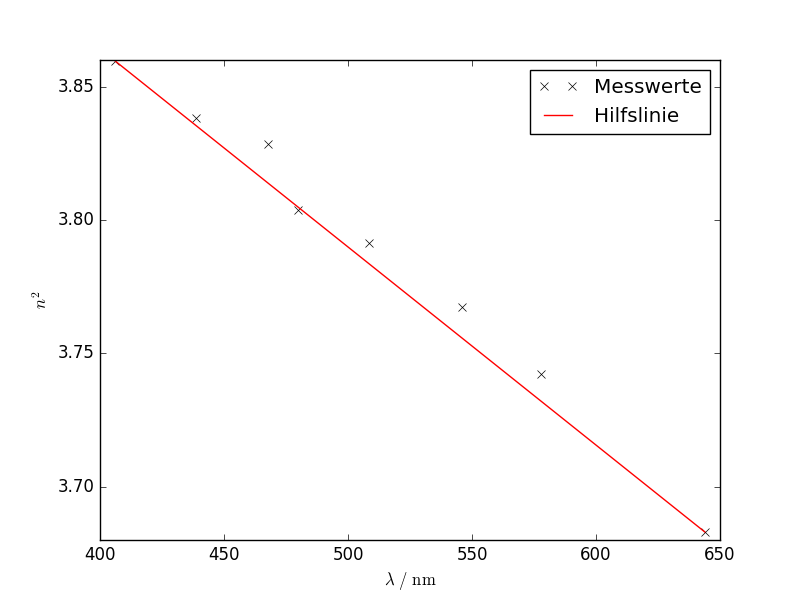
\includegraphics[width=0.8\textwidth]{Tendenz.png}
	\caption{Graphik zur Abschätzung, ob die Absorptionsstelle größer oder kleiner als das betrachtete Spektrum ist}
\end{figure}

\begin{table}[h!]
	\centering
	\begin{tabular}{c|c|c}
		Größe & Wert & relativer Fehler \\
		\hline
		$A_2'$ & \SI{2.2+-3.6e-25}{\meter^{-2}}
 & \SI{-0.03}{\meter^{-2}}

		\\
		$A_2$ & \SI{-2.3+-2.8e-14}{\meter\squared}
 & \SI{-0.13}{\meter\squared}
 \\
		$A_0'$ & \SI{3.31+-0.11}{}
 & \SI{0.03}{}

		\\
		$A_0$ & \SI{4.321+-0.024}{}
 & \SI{0.03}{}
 \\
		\hline
		$s'^2(A_0',A_2')$ & \SI{0.08+-0.14}{}
 & \\
		$s^2(A_0,A_2)$ & \SI{5.371e-14}{}
 & \\
	\end{tabular}
	\caption{Durch die lineare Regression berechnete Werte $A_0,A_0',A_2,A_2'$ mit Fehlern und relativen Fehlern, sowie die quadratischen Abweichungen $s^2,s'^2$ der Regressionsgeraden zu den Datenpunkten}
\end{table}
Dispersionskurve
\[ n(\lambda) = \sqrt{3.47 - \SI{1.6e-14}\lambda^{-2}} \]
\begin{figure}[h!]
	\centering
	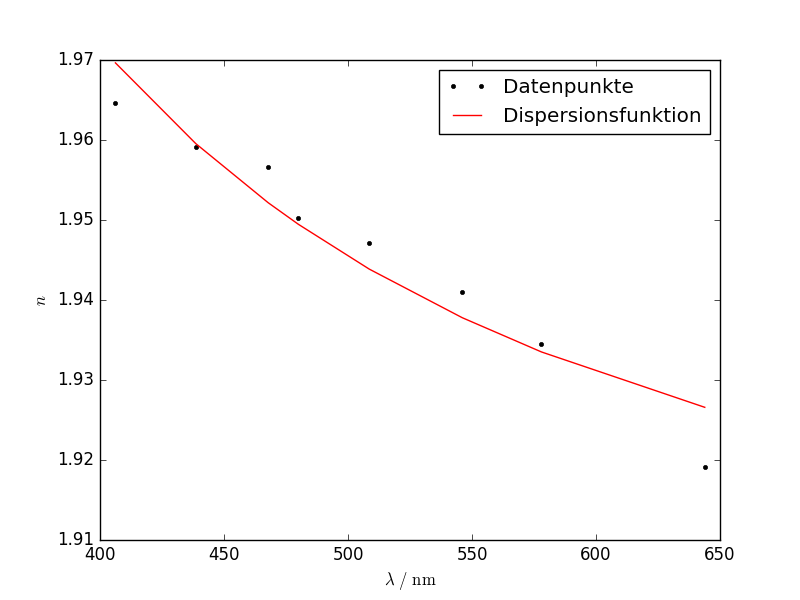
\includegraphics[width=0.8\textwidth]{Dispersionskurve.png}
	\caption{Dispersionskurve}
	\label{fig:DispKurve}
\end{figure}


Abbesche Zahl \[ \nu = \SI{-70.789}{}
 \]

Auflösungsvermögen
\begin{table}
	\centering
	\begin{tabular}{c|c}
		Wellenlänge in \si{\nano\meter} & Auflösungsvermögen \\
		\hline
		406.2 & 3810 \\
438.7 & 3017 \\
467.8 & 2481 \\
480.0 & 2296 \\
508.6 & 1927 \\
546.1 & 1554 \\
578.0 & 1308 \\
643.9 & 945  \\

	\end{tabular}
	\caption{Auflösungsvermögen bei verschiedenen Wellenlängen}
\end{table}

Absorptionsstelle \[ \lambda_1 = \sqrt{\frac{A_2}{A_0-1}} = \SI{9.664e-8}{\nano\meter}
 \]


\clearpage


\begin{table}
\centering
\begin{tabular}{c|c|c}
	Farben & Quecksilber & Cadmium \\
	\hline
	violett1 & 407.78 / 404.66 & \\
	violett2 & 435.84 & 441.46 \\
	blau &  & 467.82 \\
	türkis & 491.60 & 479.99 \\
	grün & 546.07 & \\
	gelb & 579.07 / 576.95 & \\
	orange &  & 635.99 \\
	rot &  & 643.85 \\
\end{tabular}
\end{table}
Walcher: \\
Cadmium \\
643.85	rot			stark \\
635.99	gelbrot		schwach \\
508.58	grün		stark \\
479.99	blaugrün	stark \\
467.82	blau		stark \\
441.46	blau		mittel \qquad haben wir als violett gesehen \\
\ \\
Quecksilber \\
708.19	rot			schwach \\
690.72	rot			schwach \\
579.07 und 576.95	gelb		sehr stark \\
546.07	grün		stark \\
491.60	blaugrün	mittel \\
435.84	blau		stark \qquad haben wir als violett gesehen \\
407.78 und 404.66	violett		mittel \\